\subsection{Numerical results}
We used equation \eqref{e9} to obtain first non-stationary numerical result using \texttt{Octave} function \texttt{ode45}, that solve equation with the well known explicit Runge–Kutta method of order (4,5).  The point here was to make a first step to a better understanding of the roles of the different parameters of our equation that seem of interest to us, \textit{i.e.} the resistance $R$ and the permeability $L_p$. We also aim at comparing the behaviour of IOP on different patient profile. 


For sake of simplicity we focus on patient arterial pressure. We consider three arterial pressure profile : a low arterial blood pressure  (LBP) of $26.6$, a normal arterial blood pressure (NBP) of $31.1$, and a high blood arterial pressure (HBP) of $35.5$.

We take physiological datas from the literature \textcolor{red}{INSERER CITATION Lyubimov et al, 2007,Anders, 1975,The mechanism of aqueous humour
formation,2002 \cite{•}}, and our initial values in physiological range. As it is a first step to simulation, we decide to neglect here the oscillating component. 

\begin{figure}[htbp]
 \centering
  \subfigure[Time evolution of IOP\label{fig:IOPt}]{
    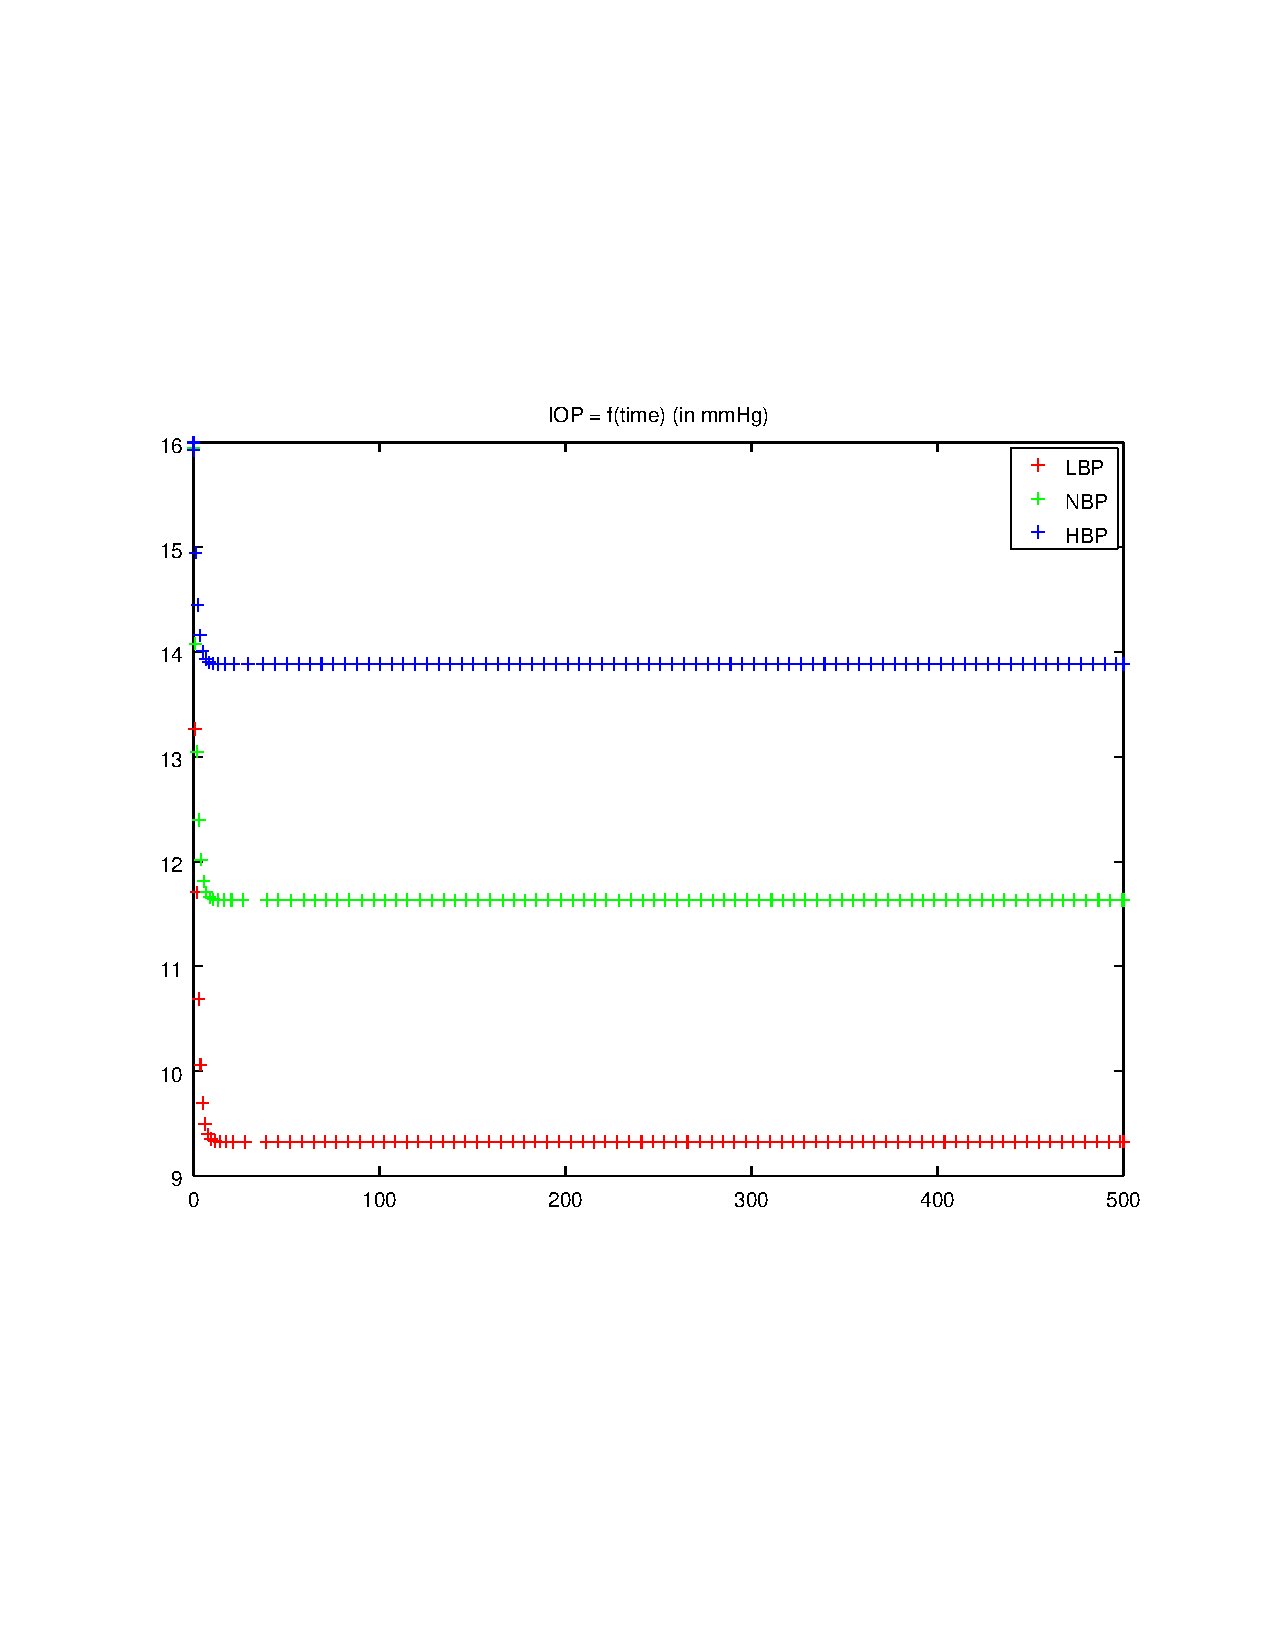
\includegraphics[width=0.45\textwidth]{images/IOP_time}
  }
  \subfigure[Time evolution of $C_2$\label{fig:C2t}]{
   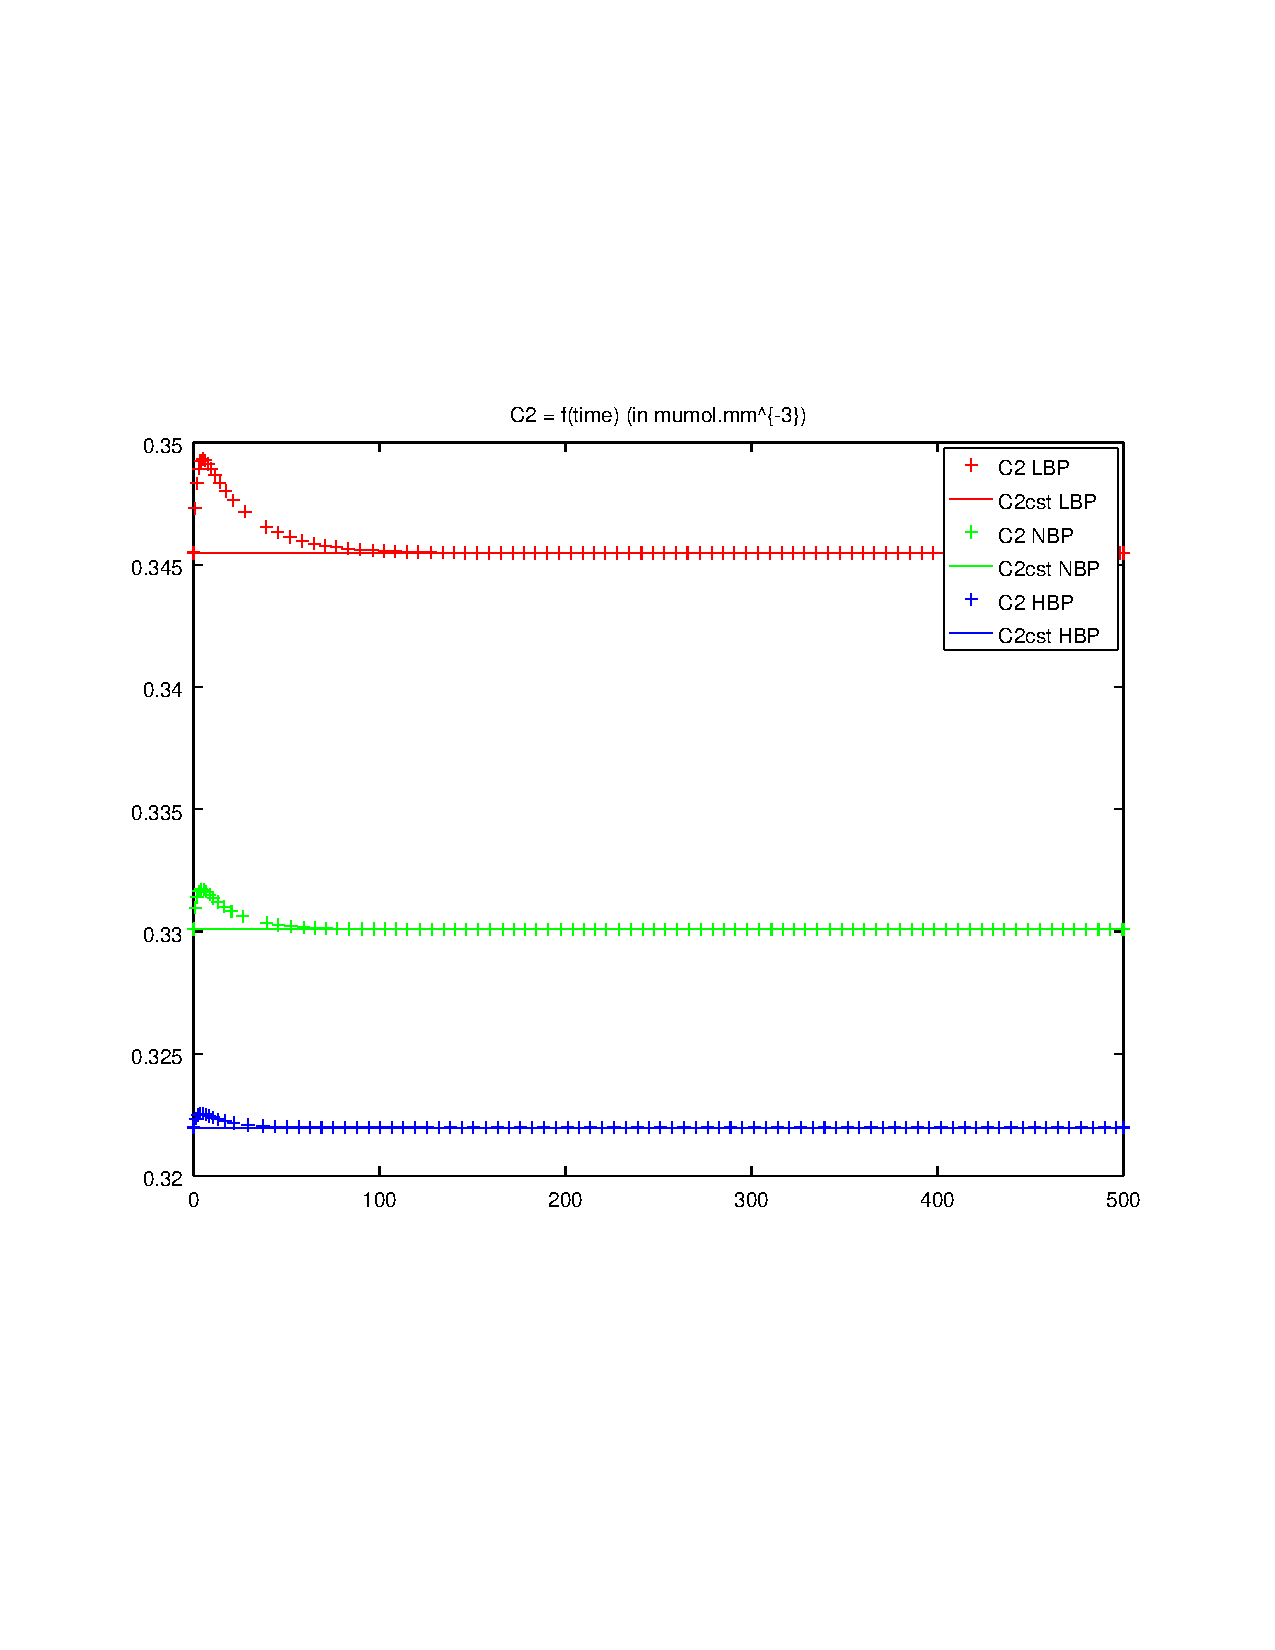
\includegraphics[width=0.45\textwidth]{images/C2_time}
 }
 
  \caption[text1]{Time evolution of IOP and $C_2$ }
    \label{fig:tevolpc2}
\end{figure}


\input 
